\section{Robustness: Feature Selection Among Significant-$\hat{\kappa}$ Stocks}\label{app:robustness_sig_kappa}

One might be concerned that the feature selection patterns documented in Section~\ref{sec:empirical} are driven by the large mass of low-volatility stocks for which the LASSO never selects any predictor.
To address this, we repeat the analysis of Section~\ref{subsec:empirical_belief_anatomy} restricting to the 155 stocks with a statistically significant $\hat{\kappa}$ estimate at the 5\% level.

The feature ranking is essentially unchanged.
The correlation between per-feature mean selection rates in the full sample and in the significant-$\hat{\kappa}$ subsample is $0.89$, and 7 of the top 10 features are identical across the two groups.
The top three features---\textit{Announce plan}, \textit{Financial reports}, and \textit{Germany}---are the same in both samples.
The Gini coefficient rises modestly from $0.18$ to $0.20$, reflecting a slight increase in concentration, but the overall distribution remains dispersed.
The macro-financial series show no systematic premium or discount relative to news topics in the restricted sample.

\paragraph{Persistence.}
We repeat the persistence analysis of Section~\ref{subsec:empirical_belief_anatomy} on the same 155 significant-$\hat{\kappa}$ stocks.
The results are nearly identical to the full sample.
Pooled across 69{,}760 selection episodes, the median run length is 4 windows and the 95th percentile is 78 windows, with a maximum of 481.
The survival curve declines from 73\% after one window to 18\% after 20 windows.
The first-order autocorrelation of the binary selection indicator, averaged across 9{,}708 active stock--feature pairs, is 0.89, decaying to 0.72 at lag 5 and 0.46 at lag 20.
Figure~\ref{fig:persistence_sig_kappa} plots the run-length distribution and survival curve for this subsample.

\begin{figure}[h]
    \centering
    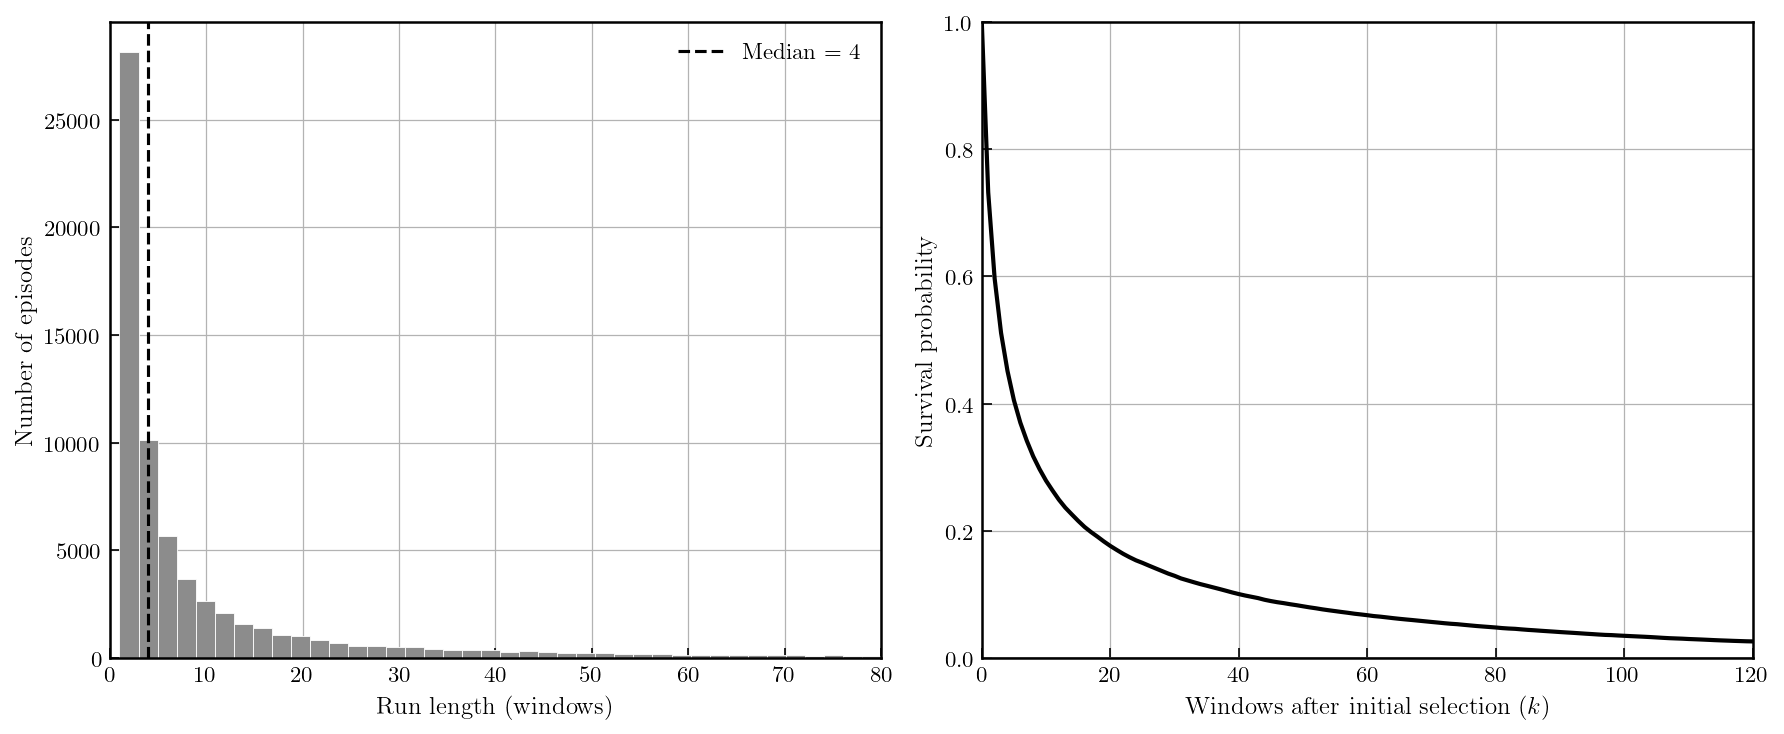
\includegraphics[width=\textwidth]{persistence_sig_kappa.png}
    \caption{Persistence of Topic Selection Episodes: Significant-$\hat{\kappa}$ Stocks}
    \label{fig:persistence_sig_kappa}
    \begin{minipage}{\textwidth}
    \footnotesize
    \textit{Note:} Same as Figure~\ref{fig:topic_selection_persistence} but restricted to the 155 stocks with a statistically significant $\hat{\kappa}$ estimate at the 5\% level.
    \textbf{Left panel}: run-length distribution truncated at 80 windows; dashed line marks the median ($=4$).
    \textbf{Right panel}: survival curve $P(\text{selected at }t+k \mid \text{selected at }t)$.
    \end{minipage}
\end{figure}

\subsection{Multiple-Testing Adjustments for Second-Stage Significance}\label{app:multiple_testing}

Because the second-stage ALM is estimated stock by stock, a natural concern is that some statistically significant $\hat{\kappa}_i$ estimates may arise from multiple testing rather than from systematic evidence in favour of the model.
To address this, we re-evaluate second-stage significance using the full set of 1{,}117 stocks for which a finite $\hat{\kappa}_i$ $t$-statistic is available in the baseline estimation output.
This is the broadest feasible comparison set for standard multiplicity corrections, because it includes every stock for which the nonlinear second-stage estimator returns a usable test statistic.

\begin{table}[H]
\centering
\caption{Multiple-Testing Corrections for Second-Stage $\hat{\kappa}_i$ Significance}
\label{tab:multiple_testing}
\begin{tabular}{lcc}
\toprule
Correction method & Rejections & Share of 1,117 tests \\
\midrule
Unadjusted 5\% level & 111 & 9.9\% \\
Benjamini--Hochberg FDR 10\% & 69 & 6.2\% \\
Benjamini--Hochberg FDR 5\% & 55 & 4.9\% \\
Holm--Bonferroni 5\% & 38 & 3.4\% \\
\bottomrule
\end{tabular}
\medskip
\begin{minipage}{0.92\textwidth}
\footnotesize
\textit{Note:} The table reports the number of second-stage ALM estimates for which the null $\kappa_i = 0$ is rejected after applying alternative multiple-testing adjustments to the 1{,}117 stocks with a finite $\hat{\kappa}_i$ $t$-statistic in the baseline estimation output. The Benjamini--Hochberg procedure controls the false discovery rate, while Holm--Bonferroni controls the family-wise error rate.
\end{minipage}
\end{table}

Table~\ref{tab:multiple_testing} shows that the number of significant second-stage estimates falls materially once multiplicity is taken into account, but a non-trivial subset of stocks remains significant even under conservative adjustments.

We also conduct a global excess-significance test.
Under the joint null that each stock-level test rejects with probability 5\%, the expected number of rejections among 1{,}117 tests is 55.9.
The observed count of 111 is almost exactly double that benchmark.
An exact binomial test for excess significance rejects strongly, with $p = 1.21 \times 10^{-11}$.
This result indicates that the aggregate number of significant second-stage estimates is too large to be explained by independent 5\% false positives alone.

The interpretation of these corrections is therefore nuanced.
They do not support reading every stock-level rejection as equally strong evidence for the model, and they imply that the raw count of unadjusted significant $\hat{\kappa}_i$ estimates overstates the amount of stock-by-stock evidence.
At the same time, the corrected results do not collapse to zero: depending on the criterion, between 38 and 69 stock-level rejections survive, and the global excess-significance test rejects decisively.
Taken together, these robustness checks suggest that the empirical support for the CMCE mechanism is concentrated in a smaller subset of stocks than the unadjusted 5\% count implies, but that the overall evidence is not well described as a pure multiple-testing artefact.
